\section{Domain model}
For at skabe et overblik over forskellige relationer, attributter og multiplisiteter, 
har gruppen valgt at lave en domænemodel.
Domænemodellen sikrer at gruppen har en repræsentation af de klasser, som skaber det domæne systemet berører.\\

Domænemodellen kan ses på figur (\ref{fig:domain})

\begin{figure}[H]
    \centering
    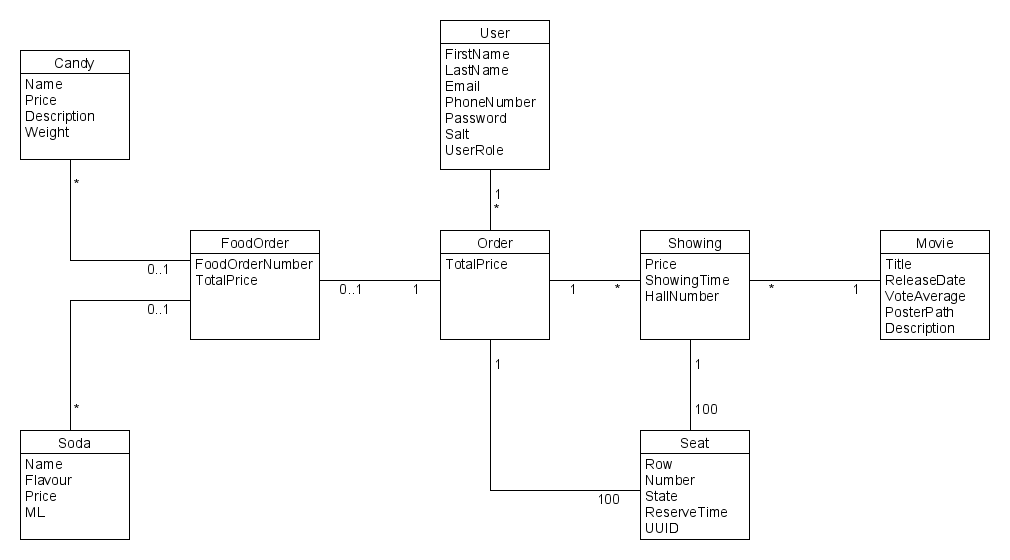
\includegraphics[width=1\textwidth]{figures/Domainmodel.png}
    \caption{Domænemodel}
    \label{fig:domain}
\end{figure}

Domænemodellen er udarbejdet over flere iterationer, og er derfor blevet ændret en del gange.
Venstre side af modellen er ikke blevet implementeret (fra FoodOrder), 
da gruppen har ikke havde mere tid til at starte på nye user stories. 
Gruppen har nået at udvikle en stor story, nemlig "Create Booking", 
som resten af domænemodellen beskriver. Storien som gruppen har udviklet er "Create Booking" 
hvilket giver kunden den største forretningsværdi.  \\

Gruppen har på 2. semester arbejdet med trelags arkitektur, og brugt det i det daværende projekt.
Herfor har det givet god mening at bygge det nuværende systemet op efter nogle af de samme principper.
Eftersom undervisningen er blevet mere kompleks, og gruppens evner er blevet udvidet, er systemet endt op med en
N-Tier arkitektur.\\